\section{Imagen de una función de dos variables}

\begin{ejercicio}
    Calcular la imagen de la función $f: A \to \bb{R}$, donde
    \begin{equation*}
        A = \{(x,y)\in \bb{R}^2\mid x^2\leq 2y-y^2\}
        \qquad \text{y} \qquad
        f(x,y)=x^2+y(y^3-4)
    \end{equation*}

    Veamos en primer lugar el conjunto en el que está definido, $A$:
    \begin{equation*}
        \begin{split}
            A &= \{(x,y)\in \bb{R}^2\mid x^2\leq 2y-y^2\}
            = \{(x,y)\in \bb{R}^2\mid x^2- 2y+y^2\leq 0\} =\\
            &= \{(x,y)\in \bb{R}^2\mid x^2 + (y-1)^2\leq 1\} =\\
            &= \ol{B}[(0,1),1]
        \end{split}
    \end{equation*}
    \begin{figure}[H]
        \centering
        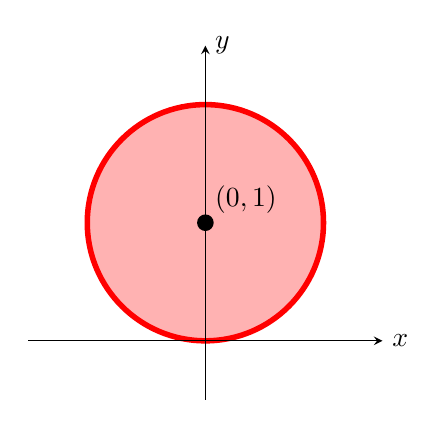
\begin{tikzpicture}[scale=1.5]
            % Círculo
            \draw[fill=red!30, draw=red, line width=2pt] (0,1) circle [radius=1];
            
            % Punto central
            \fill (0,1) circle [radius=2pt] node[above right] {$(0,1)$};

            % Ejes
            \draw[-stealth] (-1.5,0) -- (1.5,0) node[right] {$x$};
            \draw[-stealth] (0,-0.5) -- (0,2.5) node[right] {$y$};
        \end{tikzpicture}
        \caption{Conjunto de definición $A=\ol{B}[(0,1),1]$.}
    \end{figure}

    Como $A$ es una bola cerrada, tenemos que es un conjunto cerrado y acotado, luego compacto. Además, es convexo, luego conexo. Como $f$ es continua por ser polinómica, tenemos que $f(A)\subset \bb{R}$ es compacto (Teorema de Weierstrass) y conexo (Teorema del Valor Intermedio), por lo que es un intervalo cerrado y acotado, por lo que tiene mínimo y máximo.

    Estudiamos en primer lugar su interior. Tenemos que $A^\circ = B[(0,1),1]$. Como $f$ es diferenciable en todo punto de $A^\circ$ por ser polinómica, tenemos que $f$ es parcialmente derivable en todo punto $(x,y)\in A^\circ$, con:
    \begin{equation*}
        \del{f}{x}(x,y) = 2x \\
        \del{f}{y}(x,y) = 4y^3-4
    \end{equation*}
    Por tanto, los puntos críticos del interior de $A$ son aquellos que cumplen la condición necesaria de extremo relativo, $\nabla f(x,y)=0$. En este caso, el único punto crítico del interior de $A$ es el punto $(0,1)\in A^\circ$.

    Nos falta por estudiar la frontera de $A$. Tenemos que:
    \begin{equation*}
        \begin{split}
            \partial A &= \{(x,y)\in \bb{R}^2\mid x^2= 2y-y^2\}
            =\\
            &= \{(x,y)\in \bb{R}^2\mid x^2 + (y-1)^2= 1\} =\\
            &= S[(0,1),1]
        \end{split}
    \end{equation*}

    Además, como para todo $(x,y)\in A$, se tiene que $x^2 + (y-1)^2\leq 1$, entonces:
    \begin{equation*}
        (y-1)^2\leq 1 \Longrightarrow |y-1|\leq 1 \Longrightarrow y\in [0,2]
    \end{equation*}
    
    Por tanto, para $(x,y)\in \partial A\subset A$, tenemos que:
    \begin{equation*}
        f(x,y) = x^2+y(y^3-4) = 2y-y^2 + y^4-4y = y^4-y^2-2y
    \end{equation*}

    Es decir, $f(\partial A)=h([0,2])$, con $h:[0,2]\to \bb{R}$ dada por $h(y)=y^4-y^2-2y$. Calculamos por tanto la imagen de dicha función real de variable real. Como es polinómica, tenemos que $h$ es derivable en $[0,2]$, con $h'(y)=4y^3-2y-2$. Los puntos críticos son entonces los que anulan la primera derivada:
    \begin{figure}[H]
        \centering
        \polyhornerscheme[x=1]{2x^3-x-1}
    \end{figure}
    Por tanto, tenemos que $h'(y)=2(y-1)(2y^2+2y+1)$. Como $y\in [0,2]$, tenemos que el segundo factor no se anula. Por tanto, tenemos que los posibles extremos absolutos de $h$ son $\{0,1,2\}$.
    \begin{equation*}
        h(0)=0 \qquad h(1)=-2 \qquad h(2)=16-4-4 = 8
    \end{equation*}
    Por tanto, $h([0,2])=f(\partial A) = [-2,8]$.

    Como el único candidato a extremo relativo del interior de $A$ era el punto $(0,1)$, y $f(0,1)=-3$, tenemos que:
    \begin{equation*}
        f(A)=[-3,8]
    \end{equation*}
    El mínimo absoluto se da en $(0,1)$, y el máximo absoluto se da para $y=2$, es decir, para el punto $(0,2)$.
\end{ejercicio}








\begin{ejercicio}
    Calcular la imagen de la función $f: A \to \bb{R}$, donde
    \begin{equation*}
        A = \{(x,y)\in \bb{R}^2\mid (x-1)^2+y^2\leq 4,~x\geq 0\}
        \qquad \text{y} \qquad
        f(x,y)=(x-2)^2+2y^2
    \end{equation*}

    Veamos en primer lugar el conjunto en el que está definido, $A$:
    \begin{equation*}
        \begin{split}
            A &= \{(x,y)\in \bb{R}^2\mid (x-1)^2+y^2\leq 4,~x\geq 0\}
            = \ol{B}[(1,0),2]\cap (\bb{R}^+_0\times \bb{R})
        \end{split}
    \end{equation*}
    \begin{figure}[H]
        \centering
        TERMINAR
        \caption{Conjunto de definición $A$.}
    \end{figure}

    Como $A$ es la intersección de una bola cerrada (cerrado) con 
    
    Tenemos que $\bb{R}^+_0\times \bb{R}=g^{-1}([0,+\infty[)$, donde $g:\bb{R}\to \bb{R}$ dada por $g(x)=x$ es una función continua y $[0,+\infty[$ es un cerrado. Como la imagen inversa de un cerrado mediante una función continua es un cerrado, tenemos que $\bb{R}^+_0\times \bb{R}$ es un cerrado. Además, como una bola cerrada es un cerrado, tenemos que $A$ es la intersección de dos cerrados, luego es cerrado. Además, es acotado, ya que $A\subset B[(1,0), 3]$ (por ejemplo). Por tanto como es cerrado y acotado y $A\subset \bb{R}^n$, tenemos que es compacto. 

    Además, una bola cerrada es convexa, y el semiplano $x\geq 0$ también es convexo, luego su intersección es convexa, luego conexa. 
    
    Como $f$ es continua por ser polinómica, tenemos que $f(A)\subset \bb{R}$ es compacto (Teorema de Weierstrass) y conexo (Teorema del Valor Intermedio), por lo que es un intervalo cerrado y acotado, por lo que tiene mínimo y máximo.

    Estudiamos en primer lugar su interior. Tenemos que $A^\circ = B[(1,0),2]$. Como $f$ es diferenciable en todo punto de $A^\circ$ por ser polinómica, tenemos que $f$ es parcialmente derivable en todo punto $(x,y)\in A^\circ$, con:
    \begin{equation*}
        \del{f}{x}(x,y) = 2(x-2) \\
        \del{f}{y}(x,y) = 4y
    \end{equation*}
    Por tanto, los puntos críticos del interior de $A$ son aquellos que cumplen la condición necesaria de extremo relativo, $\nabla f(x,y)=0$. En este caso, el único punto crítico del interior de $A$ es el punto $(2,0)\in A^\circ$.

    Nos falta por estudiar la frontera de $A$. Tenemos que:

    TERMINAR
\end{ejercicio}


\begin{ejercicio}[Prueba DGIIM 2022-23 y 2023-24\footnote{Se repitió ambos años}]
   Calcular la imagen de la función $f:A\to \bb{R}$, siendo
   \begin{gather*}
       A = \{(x,y)\in \bb{R}^2\mid 0\leq x \leq 2(1-y^2)\} \\
       f(x,y)=(x-1)^4 + y^2 \qquad \forall (x,y)\in A
   \end{gather*}
\end{ejercicio}